\documentclass{article}
\usepackage{mathtools}
\usepackage{amsfonts}
\usepackage{amssymb}
\usepackage{tabu}
\usepackage{commath}
\usepackage{tikz}
\usetikzlibrary{decorations.pathreplacing}
\usepackage[section]{placeins}
\usepackage{nth}
\usepackage{xspace}

\newcommand{\main}{\texttt{main.cpp}\xspace}
\newcommand{\comm}{\texttt{comm.cpp}\xspace}
\newcommand{\utils}{\texttt{utils.cpp}\xspace}
\newcommand{\timer}{\texttt{timer.cpp}\xspace}
\newcommand{\inputdeck}{\texttt{input.deck}\xspace}
\newcommand{\kineticdeck}{\texttt{kinetic.deck}\xspace}
\newcommand{\floor}{\ensuremath{\mathtt{c\_floor}}\xspace}
\newcommand{\quadorder}{\ensuremath{\mathtt{quadOrder}}\xspace}
\newcommand{\momopt}{\texttt{momopt}\xspace}
\newcommand{\dn}{\texttt{dn}\xspace}
\newcommand{\integer}{\texttt{int}\xspace}
\newcommand{\bool}{\texttt{bool}\xspace}
\newcommand{\float}{\texttt{float}\xspace}
\newcommand{\double}{\texttt{double}\xspace}
\newcommand{\chars}{\texttt{char[]}\xspace}
\newcommand{\N}{\ensuremath{\mathbb{N}}\xspace}
\newcommand{\Z}{\ensuremath{\mathbb{Z}}\xspace}
\newcommand{\Q}{\ensuremath{\mathbb{Q}}\xspace}
\newcommand{\R}{\ensuremath{\mathbb{R}}\xspace}
\newcommand{\C}{\ensuremath{\mathbb{C}}\xspace}
\newcommand{\assign}{\ensuremath{\mathrel{\texttt{:=}}}}
\DeclareMathOperator{\minmod}{minmod}
\DeclareMathOperator{\slopefit}{slopefit}
\DeclareMathOperator{\sgn}{sgn}

\newcommand{\integral}[1]{\ensuremath{\langle #1 \rangle}}
\newcommand{\closure}[1]{\ensuremath{\mathcal{E}(#1)}}
\newcommand{\twosphere}{\ensuremath{\mathbb{S}^2}\xspace}
\newcommand{\threespace}{\ensuremath{\mathbb{R}^3}\xspace}
\newcommand{\kinetic}{\texttt{kinetic}\xspace}
\newcommand{\moment}{\texttt{moment}\xspace}

\frenchspacing
\raggedright

\title{Design Document}
\author{C. Kristopher Garrett, Timothy Shaffer}

\begin{document}
\maketitle

\section{Problems Being Solved}
This software simulates particles with unit speed that scatter isotropically from
an infinite background medium according to a simple kinetic equation. External sources
are not included, but could be added in the future. The equation governing particle
behavior takes the form
\begin{align}
    \label{eqn:kinetic}
    \partial_t f + \Omega \cdot \nabla_x f + \sigma_T f =
    \frac{\sigma_S}{4\pi} \integral{f}
\end{align}
where $x \in \threespace$ is position, $\Omega \in \twosphere$ (the unit sphere)
is the direction of travel, $\sigma = \sigma(x)$ is the scattering cross section, and
\integral{\cdot} is shorthand for integration over \twosphere.

The \kinetic solver directly computes solutions to
Equation~\ref{eqn:kinetic}, while the \moment solver calculates solutions based on
the spherical harmonic basis functions. This program explicitly computes approximate
solutions to Equation~\ref{eqn:kinetic} as
the system evolves from one of several initial conditions, defined in
Section~\ref{sec:initcond}.

\section{Initial Conditions}
\label{sec:initcond}
At the beginning of simulation, the grid is initialized according to one of several
configurations. In the Gaussian initial condition, a two dimensional Gaussian function
is placed with its peak at the center of the grid. The $\sigma$ value is provided as
a configuration option to the program. The limiting case, when $\sigma=0$, is the
Delta initial condition. For this condition, the centermost cell is set to
$\frac{1}{\Delta x \Delta y}$ where $\Delta x$ and $\Delta y$ are the cell
dimensions. The Lattice initial condition corresponds to a checker board pattern of highly scattering and highly absorbing regions. This configuration is reminiscent of a
small section of a nuclear reactor core. The Lattice initial condition leaves the
grid initially empty, but has the most complicated scattering pattern of the initial
conditions. The Smooth initial condition is primarily intended for testing convergence.
This configuration initializes the grid points with a periodic boundary given by
\begin{align}
1 + \sin(2\pi x)\cos(2\pi y).
\end{align}

\section{\kinetic Solver}
The \kinetic solver is an implementation of the discrete ordinates method, also known
as $\mathrm{S}_N$.
This method uses Gauss-Legendre quadrature sets on the unit sphere. Let
$\{\Omega_1, \dots, \Omega_Q\} \in \twosphere$ be be a set of nodes with
corresponding weights $\{w_1, \dots, w_Q\}$. Then from Equation~\ref{eqn:kinetic}
\begin{equation}
    \partial_t f_q + \Omega_q \cdot \nabla_x f_q + \sigma_t f_q=
    \frac{\sigma_s}{4\pi} \sum_{q'=1}^Q w_{q'} f_{q'},
\end{equation}
where $f_q(x,t) \approx f(x, \Omega_q, t)$ for $q = 1, \dots, Q$.

This implementation uses Heun's method to achieve second order convergence. Edge values
are computed via upwinding. For approximate slopes, the double minmod limiter is used.
\section{\moment Solver}
The \moment solver uses spectral methods with Equation~\ref{eqn:kinetic}. The real
spherical harmonics serve as an orthonormal basis for $L^2$. Let
$\mathbf{m}(\Omega) =
(Y_{0,0}, Y_{1,-1}, Y_{1,0}, Y_{1,1}, \dots, Y_{N,-N}, \dots, Y_{N,N})^T$
be a vector of spherical harmonics up to and including degree $N$. The the moments
with respect to $\mathbf{m}$ are given by
\begin{equation}
    \mathbf{u}(\mathbf{x}, t) =
    \integral{\mathbf{m}(\Omega) f(\mathbf{x}, \Omega, t)}
\end{equation}
since $u_{\ell,m} = f_{\ell,m}$ and the collision operator is diagonalized.
The exact moment system is given by
\begin{equation}
    \partial_t \mathbf{u} + \nabla_x \cdot \integral{\Omega\mathbf{m}f} =
    \Dif \mathbf{u},
\end{equation}
but this formulation is not closed. Thus $f$ is replaced with a $\mathrm{P}_N$
moment closure $\closure{\mathbf{u}}$ such that
$\integral{\mathbf{m}\closure{\mathbf{u}}} = \mathbf{u}$. In this case,
\begin{equation}
    \closure{\mathbf{u}} = \sum_k u_k m_k = \mathbf{u}^T \mathbf{m}
\end{equation}
yielding the closed moment system
\begin{equation}
    \partial_t \mathbf{u} + \nabla_x \cdot
    \integral{\Omega\mathbf{m}\closure{\mathbf{u}}} = \Dif \mathbf{u}.
\end{equation}

It is only necessary to use the spherical harmonics $Y_{\ell,m}$ such that
$\ell + m$ is even.

Various filters can also be applied to suppress oscillations in spherical harmonics.
These filters scale the moments on each time step. 
\subsection{Hauck Filter}
Let $N$ be the moment order and $\omega$ be the filter tune, and define
\begin{equation}
    \alpha = \frac{\omega}{N^2 (\sigma_T L + N)^2}.
\end{equation}
Scale each moment by
\begin{equation}
    \frac{1}{1 + \alpha n^2 (n+1)^2}
\end{equation}
for the $n$\textsuperscript{th} moment.

\subsection{Sspline Filter}
With moment order $N$ and filter tune $\sigma_e$, let
\begin{equation}
    s = \frac{-\sigma_e \Delta t}{\log F(N/(N+1))}
\end{equation}
where $F(x) = 1/(1 + x^4)$. The scale factor is given by
\begin{equation}
    F(n/(N+1))^s.
\end{equation}

\subsection{Lanczos Filter}
Again with moment order $N$ and filter tune $\sigma_e$, let
\begin{equation}
    s = \frac{-\sigma_e \Delta t}{\log L(N / (N+1))}
\end{equation}
where
\begin{equation}
    L(x) = \begin{dcases*}
        1 & when $x=0$ \\
        \frac{\sin x}{x} & otherwise.
    \end{dcases*}
\end{equation}
Now the moment scale factor is
\begin{equation}
    L(n / (N+1))^s.
\end{equation}

\begin{itemize}
\item Write Kinetic Equation
\item Write Initial Conditions
\item Write Approximations/Solvers
\end{itemize}


\section{Installation}
TBD

\section{Source Files}
\label{src}
\subsection{\main}
\label{src:main.cpp}
For this, I don't think we need this much info.
Just put something like
\begin{itemize}
\item \texttt{main.cpp} -- Entry point of program
\item \texttt{comm.cpp} -- Controls MPI communication
\item etc...
\end{itemize}


The main entry point for the program, \main, is responsible for reading the input
files dictating runtime behavior, setting up MPI, and running the chosen solver.
In addition, the grid initialization used by all solvers is defined here, so \main
controls the grid geometry and initial configuration. Program flow is as follows
\begin{enumerate}
    \item Determine the current node and total number of nodes. If MPI support is not
    compiled in, fall back to default values corresponding to the primary and
    only node.
    \item Read in the configuration stored in \inputdeck. This format is
    described in Section~\ref{file:input.deck}.
    \item Configure the solver. Solvers are described in Section~\ref{solver}.
    \item Set the domain of the current node.
    \item Initialize the grid.
    \item Run the solver over the specified time interval.
    \item Output data.
\end{enumerate}

The default grid initialization, \texttt{Solver::initializeGrid}, also resides
in \main. At present, all solvers use this
method. The grid is represented as a two dimensional array of floating point values.
The grids used in the program are larger than configured in \inputdeck; a border of
of a specified width of ghost cells is added outside the grid described in the
configuration.  The center points of the cells are used for calculation of
initial conditions. Figure~\ref{fig:grid} illustrates this layout.
There are two other arrays of identical size storing $\sigma_S$ and $\sigma_T$
values. To initialize the grid, first set the the border cells to the
specified floor value, \floor, and then calculate the initial values for the
main cells.

\subsubsection{Delta Initial Condition}
\label{init:delta}
When \texttt{INITCOND\_LINESOURCE} is specified with Gaussian $\sigma=0$, the
Delta Initial Condition applies. In this case, $\sigma_S$ and $\sigma_T$ for each
cell are set to $\sigma$. The cells of the initial grid are set to \floor,
with the exception of the centermost cell, %TODO check on this, not really sure
which is set to $1 / \Delta x \Delta y$ where $\Delta x$ and $\Delta y$ denote the
dimensions of each cell.

\subsubsection{Gaussian Initial Condition}
\label{init:gauss}
This condition is used when \texttt{INITCOND\_LINESOURCE} is selected as the the
initial condition and Gaussian $\sigma \neq 0$. Each cell's initial value is
set to $\max \{\texttt{gaussianFactor}, \floor\}$ where
\begin{equation}
    \mathtt{gaussianFactor} \assign \frac{1}{2\pi\sigma^2}
        \exp \left(- \frac{x_i^2 + y_j^2}{2\sigma^2}\right).
\end{equation}
$\sigma_S$ and $\sigma_T$ for each cell is set to $\sigma$.

\subsubsection{Lattice Initial Condition}
\label{init:lattice}
When \texttt{INITCOND\_LATTICE} is specified, each cell's initial value is set to
\floor, and $\sigma_S,\sigma_T \assign 1$. For any cell $(x_i,y_j)$ with
\begin{equation}
    \|(x_i,y_j) - (s_x, s_y)\|_\infty < 0.5
\end{equation}    
for some $(s_x,s_y) \in \{$
    % I don't like switching out of math mode here, but I need the line broken,
    % and since it's in a paragraph, I'll just leave it like this for now.
    (2.0,2.0), (2.0,0.0), (2.0,-2.0), (1.0,1.0), (1.0,-1.0),
    (0.0,-2.0), (-1.0,1.0), (-1.0,-1.0), (-2.0,2.0), (-2.0,0.0), (-2.0,-2.0)
$\}$, $\sigma_T$ is set to 10 and $\sigma_S$ is set to 0.

\subsubsection{Smooth Periodic Condition}
\label{init:smooth}
When \texttt{INITCOND\_PERIODIC} is selected, $\sigma_S, \sigma_T$ are initialized
to $\sigma$, and the initial value at each point $(x_I,y_j)$ is set to
\begin{equation}
    \sin(2\pi x_i) \cos(2\pi y_j) + 1.
\end{equation}

\begin{figure}
    \centering
    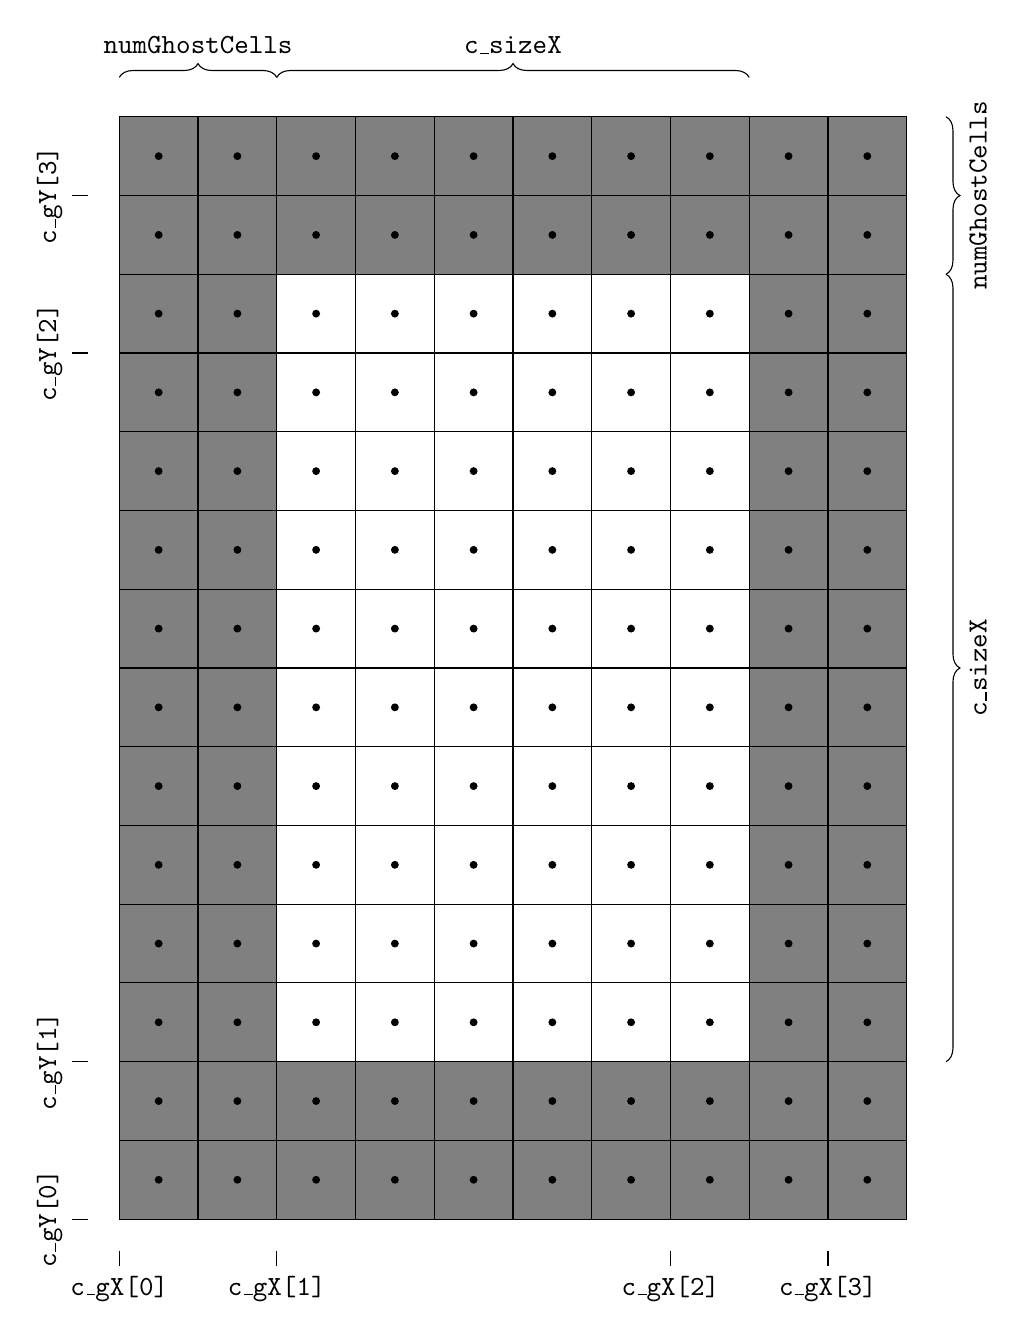
\begin{tikzpicture}[decoration={brace, amplitude=5}]
        \filldraw[fill=gray] (-5,-7) rectangle (5,7);
        \filldraw[fill=white] (-3,-5) rectangle (3,5);
        \draw[step=1] (-5,-7) grid (5,7);
        \draw[decorate] (-5,7.5) -- node[above=5] {\texttt{numGhostCells}} (-3,7.5);
        \draw[decorate] (5.5,7) -- node[rotate=90,below=5]
            {\texttt{numGhostCells}} (5.5,5);
        \draw[decorate] (-3,7.5) -- node[above=5] {\texttt{c\_sizeX}} (3,7.5);
        \draw[decorate] (5.5,5) -- node[rotate=90,below=5]
            {\texttt{c\_sizeX}} (5.5,-5);
        \draw (-5,-7.4) -- (-5,-7.6) node[below] {\texttt{c\_gX[0]}};
        \draw (-3,-7.4) -- (-3,-7.6) node[below] {\texttt{c\_gX[1]}};
        \draw (2,-7.4) -- (2,-7.6) node[below] {\texttt{c\_gX[2]}};
        \draw (4,-7.4) -- (4,-7.6) node[below] {\texttt{c\_gX[3]}};
        \draw (-5.4,-7) -- (-5.6,-7) node[above,rotate=90] {\texttt{c\_gY[0]}};
        \draw (-5.4,-5) -- (-5.6,-5) node[above,rotate=90] {\texttt{c\_gY[1]}};
        \draw (-5.4,4) -- (-5.6,4) node[above,rotate=90] {\texttt{c\_gY[2]}};
        \draw (-5.4,6) -- (-5.6,6) node[above,rotate=90] {\texttt{c\_gY[3]}};
        \foreach \x in {-4.5,-3.5,...,4.5}
        \foreach \y in {-6.5,-5.5,...,6.5}
            \fill (\x,\y) circle (0.05);
    \end{tikzpicture}

    \vspace{0.5cm}

    \caption{Grid layout}
    \label{fig:grid}
\end{figure}

\subsection{\comm}
\label{src:comm.cpp}
When using MPI, \comm communicates boundary data between nodes.
\texttt{Solver::getInnerBoundaries} is first called to obtain grid data on the
boundaries of the current node's region of the domain. Next, each node trades boundary
data with its neighbors to the north, south, east, then west via
\texttt{MPI\_Sendrecv}. Finally, the node calls \texttt{Solver::setOuterBoundaries}
to update its grid with the data from neighboring nodes.

\subsection{\utils}
\label{src:utils.cpp}
\utils is mostly comprised of IO-related utility functions. In addition, there are
functions to compute the 1-norm of an arbitrary vector and to compute Gaussian weights and nodes using GSL.

\subsection{\timer}
\label{src:timer.cpp}
\timer contains a timer class used in \main to record the time taken by computations.

\section{Solvers}
\label{solver}
All solvers must store internal parameters and grid data, and implement methods to
initialize, query grid parameters, update, and output data. See \texttt{solver.h}
for more detail. Each solver is organized into a directory containing the necessary
functionality split across several files. The solvers currently implemented
are \kinetic, \moment, \momopt, and \dn.

\subsection{\kinetic}
\label{solver:kinetic}
\subsubsection{\texttt{kinetic\_init.cpp}}
\label{src:kinetic_init.cpp}
\kinetic reads its runtime configuration from the file \kineticdeck
(see Section~\ref{file:kinetic.deck}). The maximum $\Delta t$ value \texttt{maxDt}
is calculated as
\begin{equation} %TODO check on roundabout 1/2
    \mathtt{maxDt} \assign \frac{1}{2} (\mathtt{cflFactor})
        \frac{\Delta x \Delta y}{\Delta x + \Delta y}.
\end{equation}
The grid is initialized as described in Section~\ref{src:main.cpp}. In addition to
the grid layers common to all solvers, \kinetic uses two others, \texttt{c\_kinetic}
and \texttt{c\_flux}. \utils is used
to get the quadrature as described in Section~\ref{src:utils.cpp}. These fixed-order
Gauss-Legendre integration points and weights returned will be referred to as $\mu_i$,
and $w_i$, respectively. Next, the
azimuthal angles of quadrature, $\phi_k$, are calculated as
\begin{equation}
    \phi_k \assign \frac{(k + 0.5)\pi}{\quadorder}
\end{equation}
for $k \in \Z$ such that $0 \leq k < 2(\quadorder)$,
placing $2(\quadorder)$ points evenly around the unit circle.
The quadrature weights are ultimately stored in
\texttt{c\_quadWeights}, and the points are mapped into cylindrical coordinates
and stored in \texttt{c\_xi} and \texttt{c\_eta}.
%TODO make sure geometric description is correct

For $q_1,q_2$ such that $0 \leq q_1 < (\quadorder) / 2$ and
$0 \leq q_2 < 2(\quadorder)$, define a quadrature counter
$q \assign 2(\quadorder)q_1 + q_2$. Now 
\begin{align}
    \mathtt{c\_quadWeights[q]} &\assign \frac{2\pi w_{q_1}}{\quadorder} \\
    \mathtt{c\_xi[q]} &\assign \sqrt{1 - \mu_{q_1}^2} \cos \phi_{q_2} \\
    \mathtt{c\_eta[q]} &\assign \sqrt{1 - \mu_{q_1}^2} \sin \phi_{q_2}
\end{align}

\subsubsection{\texttt{kinetic\_update.cpp}}
\label{src:kinetic_update.cpp}
The core of the \kinetic solver is the \texttt{update} method defined here. Each
call to update one time step operates as follows:
\begin{enumerate}
    \item Make a copy of the \texttt{c\_kinetic} grid.
    \item Carry out the first Euler step.
    \item Carry out the second Euler step.
    \item Average the initial grid with the results of the second iteration.
\end{enumerate}
Some preliminary functions will be used in the discussion of the above steps.

The \texttt{minmod(double x, double y)} function is designed to return
\begin{itemize}
    \item 0 if $xy < 1$
    \item $\min\{x, y\}$ if $x,y > 0$
    \item $-\min\{|x|, |y|\}$ if $x,y < 0$
\end{itemize}
and implemented as follows.
\begin{equation}
    \minmod (x, y) = \sgn'(x) \max\left(0, \min\left(|x|, y \sgn'(x)\right)\right)
\end{equation}
where
\begin{equation}
    \sgn'(x) =
    \begin{dcases*}
        1  & if $x \geq 0$ \\
        -1 & otherwise.
    \end{dcases*}
\end{equation}

Additionally,
\begin{equation}
    \slopefit(\ell, c, r, \theta) = \minmod\left((r - c)\theta,
        \minmod\left(\frac{1}{2}(r - \ell), (c-\ell)\theta\right)\right).
\end{equation}

To carry out each Euler step, the \kinetic solver first communicates the current cell's
boundaries with neighboring MPI cells (described in
Section~\ref{src:kinetic_boundaries.cpp}) and then solves flux for the
cell (described below). For each cell $(i,j)$ in the main grid (excluding the ghost
cells), the integral of $F$ is calculated as
\begin{equation}
    \texttt{integral} \assign
    \frac{\sigma_{S,(i,j)}}{4\pi} \sum_{q=0}^n w_q f_q(i,j)
\end{equation}
where $w_q$ is the calculated quadrature weight for the $q$\textsuperscript{th} point
of an $n$ point Gauss-Legendre quadrature and
$f_q(i,j)$ is the value of the \texttt{c\_kinetic} grid at $(i,j,q)$.

For each $0 \leq q < n$, subtract from the value of \texttt{c\_kinetic} at $(i,j,q)$
\begin{equation} % translate to recurrence relation?
    \Delta t \left(\sigma_{T,(i,j)} (\mathtt{c\_kinetic})_{(i,j,q)} -
    \mathtt{integral}\right).
\end{equation}
Next, if using \texttt{INITCOND\_LATTICE}, with the cell's bottom left point
$(x_i,y_j)$ add an additional $\Delta t$ to \texttt{c\_kinetic} at $(i,j,q)$ if
$\|(x_i,y_j)\|_\infty < 0.5$. Finally, subtract $\Delta t (\mathtt{c\_flux})_{i,j,q}$
from \texttt{c\_kinetic} at $(i,j,q)$.

Communicating boundaries, solving flux, and evaluating an Euler step are carried out
again as above. Now for each $(i,j)$ in the main grid, $0 \leq q < n$, average
\texttt{c\_kinetic} at $(i,j,q)$ with the corresponding cell from the copy made at
the beginning of the procedure.

Solving for flux involves approximating the flux in each of four directions
(north, south, east, west) using
\texttt{slopefit} applied to the current cell and its neighbors. The overall flux for
each cell is then calculated as
\begin{equation}
    \frac{\xi_q}{\Delta x} (\mathtt{eastFlux} - \mathtt{westFlux}) +
    \frac{\eta_q}{\Delta y} (\mathtt{northFlux} - \mathtt{southFlux}).
\end{equation}

\subsubsection{\texttt{kinetic\_boundaries.cpp}}
\label{src:kinetic_boundaries.cpp}
The \kinetic solver uses the code in \texttt{kinetic\_boundaries.cpp} in
conjunction with \texttt{Solver::communicateBoundaries()}
(see Section~\ref{src:comm.cpp}) to coordinate the boundaries of different nodes
when using MPI.
The methods defined here take pointers to buffers from which and into which to copy
grid data. These methods copy the north, south, east, and west parts of the gray
area as shown in Figure~\ref{fig:grid}.

\subsubsection{\texttt{kinetic\_output.cpp}}
\label{src:kinetic_output.cpp}
The \kinetic solver exports data to files named \texttt{out\_\%.3f\_\%d.sn}
formatted with the time under simulation and the node index. This file
consists of a short header recording the dimensions of the grid, the domain bounds,
and the number of quadrature points and weights. The rest of the file contains the
floating point values of \texttt{c\_kinetic} over the main grid (\emph{not}
including the ghost cells).

\section{Special Files}
\label{file}
\subsection{\inputdeck}
\label{file:input.deck}
\inputdeck is the primary input file which controls the basic operation of the program.
\inputdeck is a line-based text file storing a set of runtime configuration options
as an ordered listing of key-value pairs. An example file is included with the source
code. The required options are discussed in Table~\ref{table:input.deck}.
\begin{table}
    \centering
    \caption{Parameters for \inputdeck}
    \label{table:input.deck}

    \vspace{0.5cm}

    \begin{tabu}{c c X[l]}
        Option & Type & Description \\ \hline
        \texttt{SOLVER} & \chars &
            Solver to be used. Allowed values are \kinetic,
            \moment, \momopt, and \dn. The operation
            of each solver is discussed in Section~\ref{solver}. \\
        \texttt{NUM\_CELLS\_X} & \integer &
            Number of grid cells in the $x$ direction \\
        \texttt{NUM\_CELLS\_Y} & \integer &
            Number of grid cells in the $y$ direction \\
        \texttt{NUM\_MPI\_PARTITIONS\_X} & \integer &
            Number of MPI partitions in the $x$ direction \\
        \texttt{NUM\_MPI\_PARTITIONS\_Y} & \integer &
            Number of MPI partitions in the $y$ direction \\
        \texttt{A\_X} & \double &
            $x$ coordinate of the bottom left corner of the grid \\
        \texttt{B\_X} & \double &
            $x$ coordinate of the top right corner of the grid \\
        \texttt{A\_Y} & \double &
            $y$ coordinate of the bottom left corner of the grid \\
        \texttt{B\_Y} & \double &
            $y$ coordinate of the top right corner of the grid \\
        \texttt{T\_FINAL} & \double &
            Duration of the simulation \\
        \texttt{OUT\_DELTA\_T} & \double &
            Temporal resolution of the output files \\
        \texttt{GAUSSIAN\_SIGMA} & \double &
            $\sigma$ used in the initial grid configurations \\
        \texttt{FLOOR} & \double &
            Minimum value that occurs in the grid \\
        \texttt{INIT\_COND} & \integer &
            How the initial grid values are calculated. Allowed values are
            0, 1, and 2, corresponding to \texttt{INITCOND\_LINESOURCE},
            \texttt{INITCOND\_LATTICE}, and \texttt{INITCOND\_PERIODIC},
            respectively. Grid initialization is described in
            Section~\ref{src:main.cpp}. \\
        \texttt{SIGMA} & \double &
            Default scattering used in the $\sigma_S$ and $\sigma_T$
            grids. The scattering values for each grid position are determined
            based on the particular initial condition selected.
    \end{tabu}
\end{table}

\subsection{\kineticdeck}
\label{file:kinetic.deck}
\kineticdeck is a brief runtime configuration file controlling the behavior of the
\kinetic solver. This file uses the same format as
\inputdeck (Section~\ref{file:input.deck}). The required options are given in
Table~\ref{table:kinetic.deck}.
\begin{table}
    \centering
    \caption{Parameters for \kineticdeck}
    \label{table:kinetic.deck}

    \vspace{0.5cm}

    \begin{tabu}{c c X[l]}
        Option & Type & Description \\ \hline
        \texttt{QUAD\_ORDER} & \integer &
            Order of the Gaussian quadrature used for integration \\
        \texttt{CFL\_FACTOR} & \double &
            Parameter used to choose the maximum $\Delta t$ without violating the
            CFL~Condition.
    \end{tabu}
\end{table}
\end{document}